\begin{figure}[ht]
  \centering
  \begin{subfigure}[t]{0.25\textwidth}
    \centering
    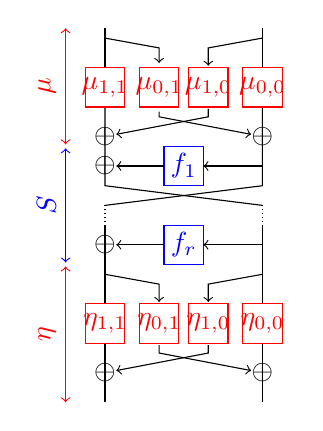
\begin{tikzpicture}[xscale=0.5,yscale=0.5]
      % Feistel functions
      \draw[color=blue]
      (-0.5, +1.5) rectangle (+0.5, +2.5) node[pos=0.5]{$f_{1}$}
      (-0.5, -0.5) rectangle (+0.5, +0.5) node[pos=0.5]{$f_{r}$};
      % branches
      \draw (-2.0, +3.5) -- (-2.0, +1.5) -- (+2.0, +1.0);
      \draw[densely dotted, black] (+2.0, +1.0) -- (+2.0, +0.5); 
      \draw (+2.0, +0.5) -- (+2.0,  -1.5);
      \draw (+2.0, +3.5) -- (+2.0, +1.5) -- (-2.0, +1.0);
      \draw[densely dotted, black] (-2.0, +1.0) -- (-2.0, +0.5); 
      \draw (-2.0, +0.5) -- (-2.0,  -1.5);
      % XORs
      \draw (-2.0, +2.0) node[inner sep=0](xor0){$\oplus$} ;
      \draw (-2.0, -0.0) node[inner sep=0](xor3){$\oplus$} ;
      % arrows
      \draw[->] (+2.0, +2.0) -- (+0.5, +2.0);
      \draw[->] (-0.5, +2.0) -- (xor0);
      \draw[->] (+2.0, -0.0) -- (+0.5, -0.0);
      \draw[->] (-0.5, -0.0) -- (xor3);
      % top whitening linear layer (mu)
      \draw (-2.0, +5.5) -- (-2.0, +4.5);
      \draw (+2.0, +5.5) -- (+2.0, +4.5);
      \draw[color=red] (-2.5, +3.5) rectangle (-1.5, +4.5) node[pos=0.5]{$\mu_{1,1}$};
      \draw[color=red] (-1.125, +3.5) rectangle (-0.125, +4.5) node[inner sep=5,pos=0.5](mu_lr){$\mu_{0,1}$};
      \draw[color=red] (+0.125, +3.5) rectangle (+1.125, +4.5) node[inner sep=4,pos=0.5](mu_rl){$\mu_{1,0}$};
      \draw[color=red] (+1.5, +3.5) rectangle (+2.5, +4.5) node[pos=0.5]{$\mu_{0,0}$};
      \draw (-2.0, +2.75) node[inner sep=0](xor_mu_l){$\oplus$};
      \draw (+2.0, +2.75) node[inner sep=0](xor_mu_r){$\oplus$};
      \draw[<-] (mu_lr) -- +(+0, +1.00) -- (-2.0, +5.25);
      \draw[->] (mu_lr) -- +(+0, -0.75) -- (xor_mu_r);
      \draw[<-] (mu_rl) -- +(+0, +1.00) -- (+2.0, +5.25);
      \draw[->] (mu_rl) -- +(+0, -0.75) -- (xor_mu_l);
      % bottom whitening linear layer (eta)
      \draw (-2.0, -4.0) -- (-2.0, -2.5);
      \draw (+2.0, -4.0) -- (+2.0, -2.5);
      \draw[color=red] (-2.5, -1.5) rectangle (-1.5, -2.5) node[pos=0.5]{$\eta_{1,1}$};
      \draw[color=red] (-1.125, -1.5) rectangle (-0.125, -2.5) node[inner sep=4,pos=0.5](eta_lr){$\eta_{0,1}$};
      \draw[color=red] (+0.125, -1.5) rectangle (+1.125, -2.5) node[inner sep=4,pos=0.5](eta_rl){$\eta_{1,0}$};
      \draw[color=red] (+1.5, -1.5) rectangle (+2.5, -2.5) node[pos=0.5]{$\eta_{0,0}$};
      \draw (-2.0, -3.25) node[inner sep=0](xor_eta_l){$\oplus$};
      \draw (+2.0, -3.25) node[inner sep=0](xor_eta_r){$\oplus$};
      \draw[<-] (eta_lr) -- +(+0, +1.00) -- (-2.0, -0.75);
      \draw[->] (eta_lr) -- +(+0, -0.75) -- (xor_eta_r);
      \draw[<-] (eta_rl) -- +(+0, +1.00) -- (+2.0, -0.75);
      \draw[->] (eta_rl) -- +(+0, -0.75) -- (xor_eta_l);
      % % Indicating the different parts
      \draw[color=red,<->] (-3.0, +2.55) -- node[sloped,above]{$\mu$}  (-3.0, +5.50) ;
      \draw[color=blue,<->] (-3.0, -0.45) -- node[sloped,above]{$S$}   (-3.0, +2.45) ;
      \draw[color=red,<->] (-3.0, -4.00) -- node[sloped,above]{$\eta$} (-3.0, -0.55) ;
    \end{tikzpicture}  
    \caption{$T = \eta \circ S \circ \mu$.}
    \label{fig.affffa-step0}
  \end{subfigure}
  \hspace{0.2cm}
  \begin{subfigure}[t]{0.33\textwidth}
    \centering
    % \begin{tikzpicture}[xscale=0.5,yscale=0.5]
    %   % Feistel functions
    %   \draw[color=blue]
    %   (-0.5, +1.5) rectangle (+0.5, +2.5) node[pos=0.5]{$f_{1}$}
    %   (-0.5, -0.5) rectangle (+0.5, +0.5) node[pos=0.5]{$f_{r}$};
    %   % branches
    %   \draw (-2.0, +3.1) -- (-2.0, +1.5) -- (+2.0, +1.0);
    %   \draw[densely dotted, black] (+2.0, +1.0) -- (+2.0, +0.5); 
    %   \draw (+2.0, +0.5) -- (+2.0,  -1.2);
    %   \draw (+2.0, +3.1) -- (+2.0, +1.5) -- (-2.0, +1.0);
    %   \draw[densely dotted, black] (-2.0, +1.0) -- (-2.0, +0.5); 
    %   \draw (-2.0, +0.5) -- (-2.0,  -1.2);
    %   % XORs
    %   \draw (-2.0, +2.0) node[inner sep=0](xor0){$\oplus$} ;
    %   \draw (-2.0, -0.0) node[inner sep=0](xor3){$\oplus$} ;
    %   % arrows
    %   \draw[->] (+2.0, +2.0) -- (+0.5, +2.0);
    %   \draw[->] (-0.5, +2.0) -- (xor0);
    %   \draw[->] (+2.0, -0.0) -- (+0.5, -0.0);
    %   \draw[->] (-0.5, -0.0) -- (xor3);
    %   % top whitening linear layer (mu)
    %   \draw (-2.0, +5.5) -- (-2.0, +4.1);
    %   \draw (+2.0, +5.5) -- (+2.0, +4.1);
    %   \draw[color=red] (-1.25, +4.3) rectangle (-0.25, +5.3) node[inner sep=4,pos=0.5](a){$a$};
    %   \draw[color=red] (-2.5, +3.1) rectangle (-1.5, +4.1) node[pos=0.5]{$b$};
    %   \draw[color=red] (+0.125, +3.1) rectangle (+1.125, +4.1) node[inner sep=4,pos=0.5](mu_rl){$c$};
    %   \draw[color=red] (+1.5, +3.1) rectangle (+2.5, +4.1) node[pos=0.5]{$d$};
    %   \draw (+2.0, +4.8) node[inner sep=0](xor_a){$\oplus$};
    %   \draw (-2.0, +2.75) node[inner sep=0](xor_mu_l){$\oplus$};
    %   \draw[<-] (mu_rl) -- +(+0, +0.90) -- (+2.0, +4.5);
    %   \draw[->] (mu_rl) -- +(+0, -0.85) -- (xor_mu_l);
    %   \draw[<-] (a) -- (-2.0, +4.8);
    %   \draw[->] (a) -- (xor_a);
    %   % bottom whitening linear layer (eta)
    %   % OLD
    %     %   \draw (-2.0, -4.0) -- (-2.0, -2.2);
    %     %   \draw (+2.0, -4.0) -- (+2.0, -2.2);
    %     %   \draw[color=red] (-1.25, -2.8) rectangle (-0.25, -3.8) node[pos=0.5](aprime){$a'$};
    %     %   \draw[color=red] (-2.5, -1.2) rectangle (-1.5, -2.2) node[pos=0.5]{$b'$};
    %     %   \draw[color=red] (+0.125, -1.2) rectangle (+1.125, -2.2) node[inner sep=4,pos=0.5](eta_rl){$c'$};
    %     %   \draw[color=red] (+1.5, -1.2) rectangle (+2.5, -2.2) node[pos=0.5]{$d'$};
    %     %   \draw (-2.0, -2.55) node[inner sep=0](xor_eta_l){$\oplus$};
    %     %   \draw (+2.0, -3.3) node[inner sep=0](xor_aprime){$\oplus$};
    %     %   \draw[<-] (eta_rl) -- +(+0, +1.00) -- (+2.0, -0.70);
    %     %   \draw[->] (eta_rl) -- +(+0, -0.85) -- (xor_eta_l);
    %     %   \draw[<-] (aprime) -- (-2.0, -3.3);
    %     %   \draw[->] (aprime) -- (xor_aprime);
    %   % NEW
    %   \draw (-2.0, -4.0) -- (-2.0, -2.2);
    %   \draw (+2.0, -4.0) -- (+2.0, -2.2);
    %   \draw[color=red] (-1.25, -2.8) rectangle (-0.25, -3.8) node[pos=0.5](aprime){$a'$};
    %   \draw[color=red] (-2.5, -1.2) rectangle (-1.5, -2.2) node[pos=0.5]{$b''$};
    %   \draw[color=red] (+0.125, -1.2) rectangle (+1.125, -2.2) node[inner sep=4,pos=0.5](eta_rl){$c''$};
    %   \draw[color=red] (+1.5, -1.2) rectangle (+2.5, -2.2) node[pos=0.5]{$d''$};
    %   \draw (-2.0, -0.85) node[inner sep=0](xor_eta_l){$\oplus$};
    %   \draw (+2.0, -3.3) node[inner sep=0](xor_aprime){$\oplus$};
    %   \draw[<-] (eta_rl) -- +(+0, -1.00) -- (+2.0, -2.70);
    %   \draw[->] (eta_rl) -- +(+0, +0.85) -- (xor_eta_l);
    %   \draw[<-] (aprime) -- (-2.0, -3.3);
    %   \draw[->] (aprime) -- (xor_aprime);
    %   % % Indicating the different parts
    %   \draw[color=red,<->] (-3.0, +2.55) -- node[sloped,above]{$\mu$}  (-3.0, +5.50) ;
    %   \draw[color=blue,<->] (-3.0, -0.45) -- node[sloped,above]{$S$}   (-3.0, +2.45) ;
    %   \draw[color=blue,<->] (+3.0, -2.40) -- node[sloped,above]{$S'$}  (+3.0, +4.40) ;
    %   \draw[color=red,<->] (-3.0, -4.00) -- node[sloped,above]{$\eta$} (-3.0, -0.55) ;
    % \end{tikzpicture}  
    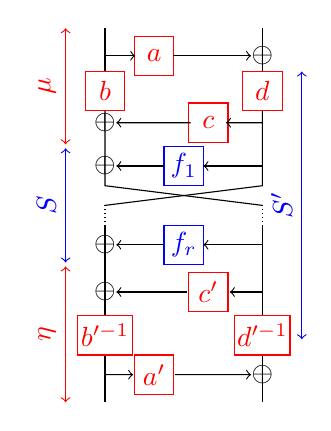
\begin{tikzpicture}[xscale=0.5,yscale=0.5]
      % Feistel functions
      \draw[color=blue]
      (-0.5, +1.5) rectangle (+0.5, +2.5) node[pos=0.5]{$f_{1}$}
      (-0.5, -0.5) rectangle (+0.5, +0.5) node[pos=0.5]{$f_{r}$};
      % branches
      \draw (-2.0, +3.4) -- (-2.0, +1.5) -- (+2.0, +1.0);
      \draw[densely dotted, black] (+2.0, +1.0) -- (+2.0, +0.5); 
      \draw (+2.0, +0.5) -- (+2.0,  -1.8);
      \draw (+2.0, +3.4) -- (+2.0, +1.5) -- (-2.0, +1.0);
      \draw[densely dotted, black] (-2.0, +1.0) -- (-2.0, +0.5); 
      \draw (-2.0, +0.5) -- (-2.0,  -1.8);
      % XORs
      \draw (-2.0, +2.0) node[inner sep=0](xor0){$\oplus$} ;
      \draw (-2.0, -0.0) node[inner sep=0](xor3){$\oplus$} ;
      % arrows
      \draw[->] (+2.0, +2.0) -- (+0.5, +2.0);
      \draw[->] (-0.5, +2.0) -- (xor0);
      \draw[->] (+2.0, -0.0) -- (+0.5, -0.0);
      \draw[->] (-0.5, -0.0) -- (xor3);
      % top whitening linear layer (mu)
      \draw (-2.0, +5.5) -- (-2.0, +4.4);
      \draw (+2.0, +5.5) -- (+2.0, +4.4);
      \draw[color=red] (-1.25, +4.3) rectangle (-0.25, +5.3) node[inner sep=4,pos=0.5](a){$a$};
      \draw[color=red] (-2.5, +3.4) rectangle (-1.5, +4.4) node[pos=0.5]{$b$};
      \draw[color=red] (+0.125, +2.6) rectangle (+1.125, +3.6) node[inner sep=4,pos=0.5](mu_rl){$c$};
      \draw[color=red] (+1.5, +3.4) rectangle (+2.5, +4.4) node[pos=0.5]{$d$};
      \draw (+2.0, +4.8) node[inner sep=0](xor_a){$\oplus$};
      \draw (-2.0, +3.1) node[inner sep=0](xor_mu_l){$\oplus$};
      \draw[<-] (mu_rl) -- (+2.0, +3.1);
      \draw[->] (mu_rl) -- (xor_mu_l);
      \draw[<-] (a) -- (-2.0, +4.8);
      \draw[->] (a) -- (xor_a);
      % bottom whitening linear layer (eta)
      \draw (-2.0, -4.0) -- (-2.0, -2.8);
      \draw (+2.0, -4.0) -- (+2.0, -2.8);
      \draw[color=red] (-1.25, -2.8) rectangle (-0.25, -3.8) node[pos=0.5](aprime){$a'$};
      \draw[color=red] (-2.7, -1.8) rectangle (-1.3, -2.8) node[pos=0.5]{$b'^{-1}$};
      \draw[color=red] (+0.125, -0.7) rectangle (+1.125, -1.7) node[inner sep=4,pos=0.5](eta_rl){$c'$};
      \draw[color=red] (+1.3, -1.8) rectangle (+2.7, -2.8) node[pos=0.5]{$d'^{-1}$};
      \draw (-2.0, -1.2) node[inner sep=0](xor_eta_l){$\oplus$};
      \draw (+2.0, -3.3) node[inner sep=0](xor_aprime){$\oplus$};
      \draw[<-] (eta_rl) -- (+2.0, -1.2);
      \draw[->] (eta_rl) -- (xor_eta_l);
      \draw[<-] (aprime) -- (-2.0, -3.3);
      \draw[->] (aprime) -- (xor_aprime);
      % % Indicating the different parts
      \draw[color=red,<->] (-3.0, +2.55) -- node[sloped,above]{$\mu$}  (-3.0, +5.50) ;
      \draw[color=blue,<->] (-3.0, -0.45) -- node[sloped,above]{$S$}   (-3.0, +2.45) ;
      \draw[color=blue,<->] (+3.0, -2.40) -- node[sloped,above]{$S'$}  (+3.0, +4.40) ;
      \draw[color=red,<->] (-3.0, -4.00) -- node[sloped,above]{$\eta$} (-3.0, -0.55) ;
    \end{tikzpicture}  
    \caption{$T$ (alt. representation).}
    \label{fig.affffa-step1}
  \end{subfigure}
  \hspace{0.2cm}
  \begin{subfigure}[t]{0.33\textwidth}
    \centering
    % \begin{tikzpicture}[xscale=0.5,yscale=0.5]
    %   % Feistel functions
    %   \draw[color=blue]
    %   (-0.5, +1.5) rectangle (+0.5, +2.5) node[pos=0.5]{$f_{1}'$}
    %   (-0.5, -0.5) rectangle (+0.5, +0.5) node[pos=0.5]{$f_{r}'$};
    %   % branches
    %   \draw (-2.0, +3.1) -- (-2.0, +1.5) -- (+2.0, +1.0);
    %   \draw[densely dotted, black] (+2.0, +1.0) -- (+2.0, +0.5); 
    %   \draw (+2.0, +0.5) -- (+2.0,  -1.2);
    %   \draw (+2.0, +3.1) -- (+2.0, +1.5) -- (-2.0, +1.0);
    %   \draw[densely dotted, black] (-2.0, +1.0) -- (-2.0, +0.5); 
    %   \draw (-2.0, +0.5) -- (-2.0,  -1.2);
    %   % XORs
    %   \draw (-2.0, +2.0) node[inner sep=0](xor0){$\oplus$} ;
    %   \draw (-2.0, -0.0) node[inner sep=0](xor3){$\oplus$} ;
    %   % arrows
    %   \draw[->] (+2.0, +2.0) -- (+0.5, +2.0);
    %   \draw[->] (-0.5, +2.0) -- (xor0);
    %   \draw[->] (+2.0, -0.0) -- (+0.5, -0.0);
    %   \draw[->] (-0.5, -0.0) -- (xor3);
    %   % top whitening linear layer (mu)
    %   \draw (-2.0, +5.5) -- (-2.0, +3.1);
    %   \draw (+2.0, +5.5) -- (+2.0, +4.1);
    %   \draw[color=red] (+1.5, +3.1) rectangle (+2.5, +4.1) node[pos=0.5]{$d$};
    %   % bottom whitening linear layer (eta)
    %   \draw (-2.0, -4.0) -- (-2.0, -1.2);
    %   \draw (+2.0, -4.0) -- (+2.0, -2.2);
    %   \draw[color=red] (+1.3, -1.2) rectangle (+2.7, -2.2) node[pos=0.5]{$d'^{-1}$};
    % \end{tikzpicture}  
    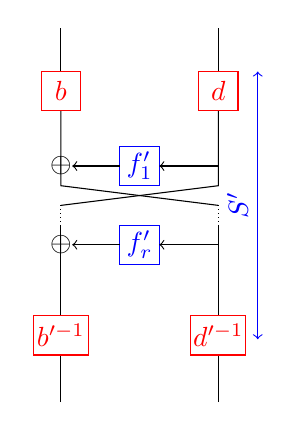
\begin{tikzpicture}[xscale=0.5,yscale=0.5]
      % Feistel functions
      \draw[color=blue]
      (-0.5, +1.5) rectangle (+0.5, +2.5) node[pos=0.5]{$f_{1}'$}
      (-0.5, -0.5) rectangle (+0.5, +0.5) node[pos=0.5]{$f_{r}'$};
      % branches
      \draw (-2.0, +3.4) -- (-2.0, +1.5) -- (+2.0, +1.0);
      \draw[densely dotted, black] (+2.0, +1.0) -- (+2.0, +0.5); 
      \draw (+2.0, +0.5) -- (+2.0,  -1.8);
      \draw (+2.0, +3.4) -- (+2.0, +1.5) -- (-2.0, +1.0);
      \draw[densely dotted, black] (-2.0, +1.0) -- (-2.0, +0.5); 
      \draw (-2.0, +0.5) -- (-2.0,  -1.8);
      % XORs
      \draw (-2.0, +2.0) node[inner sep=0](xor0){$\oplus$} ;
      \draw (-2.0, -0.0) node[inner sep=0](xor3){$\oplus$} ;
      % arrows
      \draw[->] (+2.0, +2.0) -- (+0.5, +2.0);
      \draw[->] (-0.5, +2.0) -- (xor0);
      \draw[->] (+2.0, -0.0) -- (+0.5, -0.0);
      \draw[->] (-0.5, -0.0) -- (xor3);
      % top whitening linear layer (mu)
      \draw (-2.0, +5.5) -- (-2.0, +4.4);
      \draw (+2.0, +5.5) -- (+2.0, +4.4);
    %   \draw[color=red] (-1.25, +4.3) rectangle (-0.25, +5.3) node[inner sep=4,pos=0.5](a){$a$};
      \draw[color=red] (-2.5, +3.4) rectangle (-1.5, +4.4) node[pos=0.5]{$b$};
    %   \draw[color=red] (+0.125, +2.6) rectangle (+1.125, +3.6) node[inner sep=4,pos=0.5](mu_rl){$c$};
      \draw[color=red] (+1.5, +3.4) rectangle (+2.5, +4.4) node[pos=0.5]{$d$};
    %   \draw (+2.0, +4.8) node[inner sep=0](xor_a){$\oplus$};
    %   \draw (-2.0, +3.1) node[inner sep=0](xor_mu_l){$\oplus$};
    %   \draw[<-] (mu_rl) -- (+2.0, +3.1);
    %   \draw[->] (mu_rl) -- (xor_mu_l);
    %   \draw[<-] (a) -- (-2.0, +4.8);
    %   \draw[->] (a) -- (xor_a);
      % bottom whitening linear layer (eta)
      \draw (-2.0, -4.0) -- (-2.0, -2.8);
      \draw (+2.0, -4.0) -- (+2.0, -2.8);
    %   \draw[color=red] (-1.25, -2.8) rectangle (-0.25, -3.8) node[pos=0.5](aprime){$a'$};
      \draw[color=red] (-2.7, -1.8) rectangle (-1.3, -2.8) node[pos=0.5]{$b'^{-1}$};
    %   \draw[color=red] (+0.125, -0.7) rectangle (+1.125, -1.7) node[inner sep=4,pos=0.5](eta_rl){$c'$};
      \draw[color=red] (+1.3, -1.8) rectangle (+2.7, -2.8) node[pos=0.5]{$d'^{-1}$};
    %   \draw (-2.0, -1.2) node[inner sep=0](xor_eta_l){$\oplus$};
    %   \draw (+2.0, -3.3) node[inner sep=0](xor_aprime){$\oplus$};
    %   \draw[<-] (eta_rl) -- (+2.0, -1.2);
    %   \draw[->] (eta_rl) -- (xor_eta_l);
    %   \draw[<-] (aprime) -- (-2.0, -3.3);
    %   \draw[->] (aprime) -- (xor_aprime);
      % % Indicating the different parts
    %   \draw[color=red,<->] (-3.0, +2.55) -- node[sloped,above]{$\mu$}  (-3.0, +5.50) ;
    %   \draw[color=blue,<->] (-3.0, -0.45) -- node[sloped,above]{$S$}   (-3.0, +2.45) ;
      \draw[color=blue,<->] (+3.0, -2.40) -- node[sloped,above]{$S'$}  (+3.0, +4.40) ;
    %   \draw[color=red,<->] (-3.0, -4.00) -- node[sloped,above]{$\eta$} (-3.0, -0.55) ;
    \end{tikzpicture} 
    \FigDef{afa-step2}{$S'$ (alt. representation).}
  \end{subfigure}
  \FigDef{afa-explanation}{The target of our attack, its result and its alternative representation.
  %In \FigRef{afa-step2},
  $f'_i$ is affine equivalent to $f_i$.}
\end{figure}
